%---- Sample WMSU BSMATH BEAMER template ------
%---- Begin editing after PREAMBLE END at line 77------
%---- Created by: Christle Jude L. Maquilan - April 2022 --
%---- @jmaq03.jm@gmail.com -----

\documentclass[xcolor=dvipsnames,envcountsect]{beamer}

%-------- theme --------
\usetheme{Madrid}

%-------- color --------
\definecolor{blues}{RGB}{10,100,185}
\usecolortheme[named=blues]{structure}
%-------- set color of 'example block' to crimson theme --------
\setbeamercolor{block body example}{bg=white}
\setbeamercolor{block title example}{fg=white, bg=red!50!black}

%-------- font --------
\setbeamerfont{structure}{family=\rmfamily,series=\bfseries}
\usefonttheme[stillsansseriftext]{structurebold}
\setbeamerfont{section in head/foot}{size=\tiny}

%-------- misc structure --------
\useoutertheme[footline=authortitle,subsection=false]{miniframes}
\useinnertheme{rounded}
\addtobeamertemplate{block begin}{}{\justifying}
\newtheorem{remark}[theorem]{Remark}
\renewcommand{\indent}{\hspace*{2em}}
\setbeamertemplate{theorems}[numbered]
\setbeamertemplate{caption}[numbered]
\usepackage[justification=centering]{caption}
\renewcommand{\qedsymbol}{$\blacksquare$}

%-------- packages to be used -------
\usepackage{amsmath,amsfonts,amssymb,amscd,amsthm}
\usepackage{algorithm2e}
\usepackage{algorithmic}
\usepackage{graphicx,xcolor,comment}
\usepackage{enumerate}
\usepackage{mathrsfs} 
\usepackage{multirow}
\usepackage{array}
\usepackage{hyperref}
\usepackage{multicol}
\usepackage{ragged2e}
\usepackage{caption}
\usepackage[english]{babel}
\usepackage{rotating}
\usepackage{enumerate}
\usepackage{subfigure}
\usepackage{tikz}
\usepackage{bm}
\usepackage{csquotes}
\usepackage{gensymb,textcomp,mathcomp}
\usepackage{xfrac}

\graphicspath{{Figures}}

\newcommand{\pfwd}{$\text{p}_{\text{fwd}}$}
\newcommand{\prev}{$\text{p}_{\text{rev}}$}

%-------- for bibliography -----------------
\usepackage{biblatex}
\setbeamertemplate{bibliography item}{\insertbiblabel}
\addbibresource{main1_references.bib}
\setbeamertemplate{frametitle continuation}{\frametitle{\color{white}List of References}}

%-------- WMSU Backgound -------------------
%\usebackgroundtemplate{%
%	\tikz[overlay,remember picture] \node[opacity=0.02, at=(current page.center)] {
%		\includegraphics[height=4.5in,width=4.5in]{./Figures/WMSU LOGO.png}};
%}

%---------START EDITING HERE---------------------
\title[Designing Highly Multiplex PCR Primer Sets with SADDLE]{Designing Highly Multiplex PCR Primer Sets with Simulated Annealing Design using Dimer Likelihood Estimation (SADDLE)}

\author [Xie et al. - SADDLE]{by \textbf{Nina G. Xie,  Michael X. Wang, Ping Song, Shiqi Mao, Yifan Wang, Yuxia Yang, Junfeng Luo, Shengxiang Ren, David Yu Zhang}}

\institute[Free University Berlin] {\emph{Presenter: }\textbf{Marie Hoffmann, M.Sc.}\\[1em]
	published 2022/04/11 in Nature Communications, Volume 13, Issue 1\\[1em]
%
\includegraphics[scale=0.06]{./Figures/fu_logo5.png}
}

\date[August 21, 2022]{\footnotesize\textbf{August 23, 2022}}
%--------- DURATION 30 MIN ------------------
\begin{document}
	
\begin{frame}{\titlepage}\end{frame}
\begin{frame}{\frametitle{Presentation Outline}\tableofcontents}\end{frame}
%--------- INTRODUCTION ----------------------
% \section{Introduction} 
% addresses the design of multiplex PCRs, application: NGS, qPCR
% goals of detecting species in an esample, gene fusions as observed in cancer, pathogen detection
% short: whenever there is a need to read different regions simultaneously of the same genome or mixture
\begin{frame}\frametitle{Abstract}\framesubtitle{Designing Highly Multiplex PCR Primer Sets with SADDLE}
\underline{Problem tackled}:
    \begin{itemize}
        \item Optimize primer set $S$ out of a pool of proto-primers w.r.t. low dimerization change % for tube PCRs (qPCR) limit seems to 70 primers
    \end{itemize}
\underline{Challenges}:
    \begin{itemize}
        \item Dimerization -- primer dimerization grows quadratically %with #primers
        \item Combinatorial -- exponentially many possibilities to form subset 
    \end{itemize}
\underline{Results}:
    \begin{itemize}
        \item In a 96-plex PCR primer set (192 primers), the fraction of primer dimers decreases from 90.7 \% (naively designed) to 4.9\% % scaled up to 384-plex PCR
        \item SADDLE-designed primer sets can be in NGS, but also qPCR
    \end{itemize}

	%	One major challenge in the design of highly multiplexed PCR primer sets is the large number of potential primer dimer species that grows quadratically with the number of primers to be designed. Simultaneously, there are exponentially many choices for multiplex primer sequence selection, resulting in systematic evaluation approaches being computationally intractable. Here, we present and experimentally validate Simulated Annealing Design using Dimer Likelihood Estimation (SADDLE), a stochastic algorithm for design of multiplex PCR primer sets that minimize primer dimer formation. In a 96-plex PCR primer set (192 primers), the fraction of primer dimers decreases from 90.7\% in a naively designed primer set to 4.9\% in our optimized primer set. Even when scaling to 384-plex (768 primers), the optimized primer set maintains low dimer fraction. In addition to NGS, SADDLE-designed primer sets can also be used in qPCR settings to allow highly multiplexed detection of gene fusions in cDNA, with a single-tube assay comprising 60 primers detecting 56 distinct gene fusions recurrently observed in lung cancer.
\end{frame}

\section{Background}
\begin{frame}{Field of Application: Metabarcoding}\framesubtitle{Technique}
% other qPCR - Real-time PCR as deployed for Covid testing - in tube no thermal cycler needed
\begin{multicols}{2}
\begin{itemize}
    \item Only technique capable of identifying up to thousands species/sample
    \item Affordable and well-established method % therefore interesting long-term monitoring projects involving frequent sampling
    \item Technique
    \begin{enumerate}
        \item Batch-process DNA extracts
        \item Amplify \underline{barcode} via PCR %\footnote{polymerase chain reaction}
        \item Sequence via NGS %\footnote{next-generation sequencing}
        \item Identify via match against reference database
    \end{enumerate}
\end{itemize}
% \columnbreak
    \begin{center}
        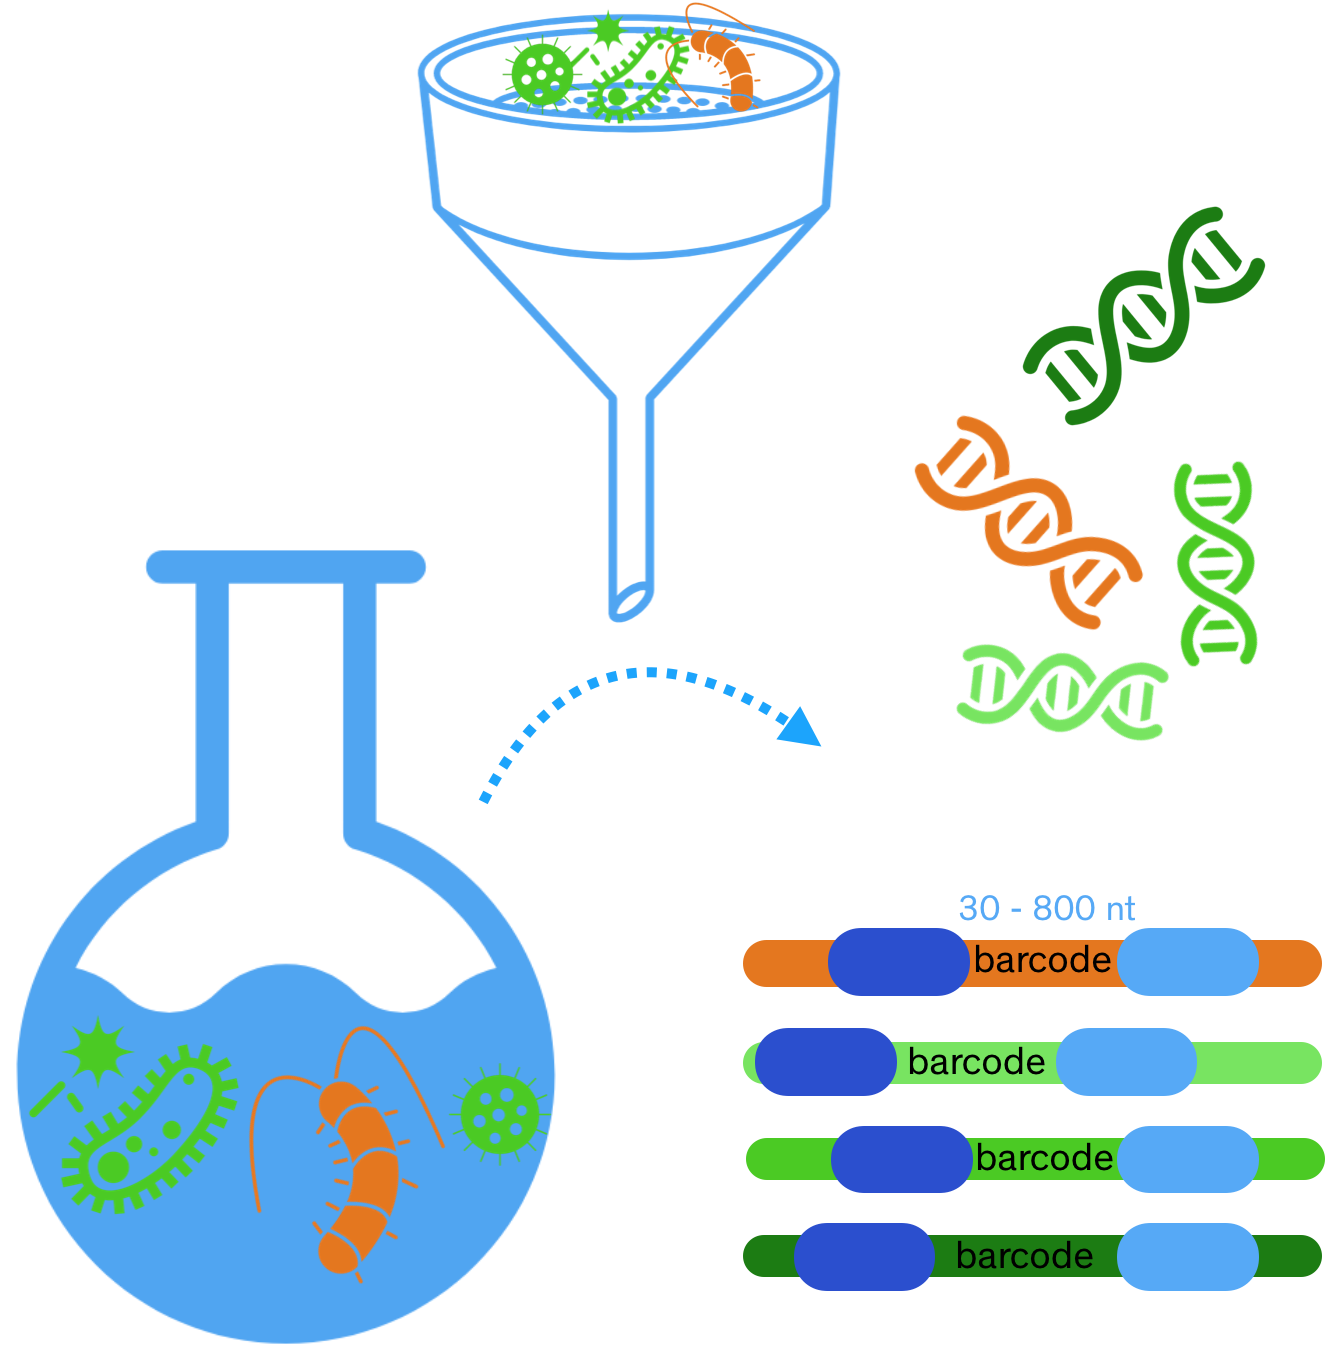
\includegraphics[width=0.5\textwidth]{picto_metabarcoding}
    \end{center}
\end{multicols}
\end{frame}

% \begin{frame}{Metabarcoding}\framesubtitle{PCR - Polymerase Chain Reaction}
%     \begin{center}
%         \only<1>{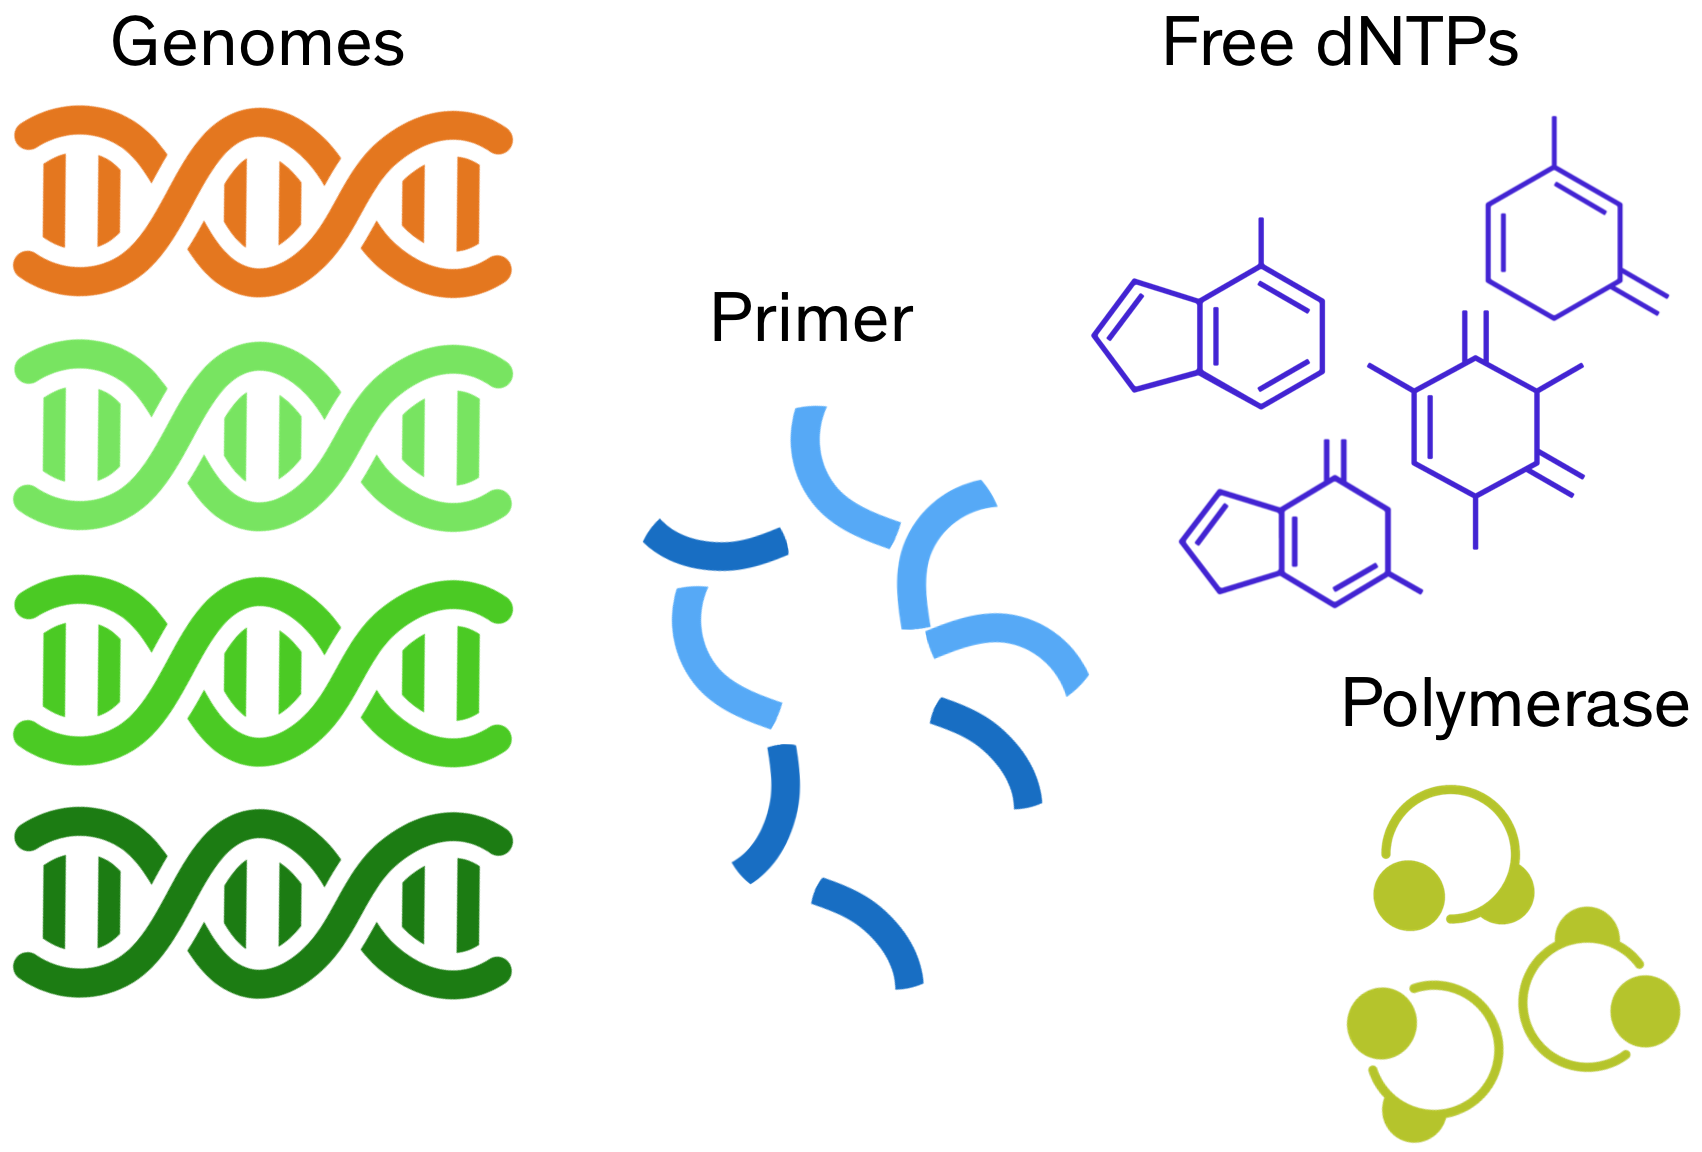
\includegraphics[scale=.32]{picto_PCR}}
%         \only<2>{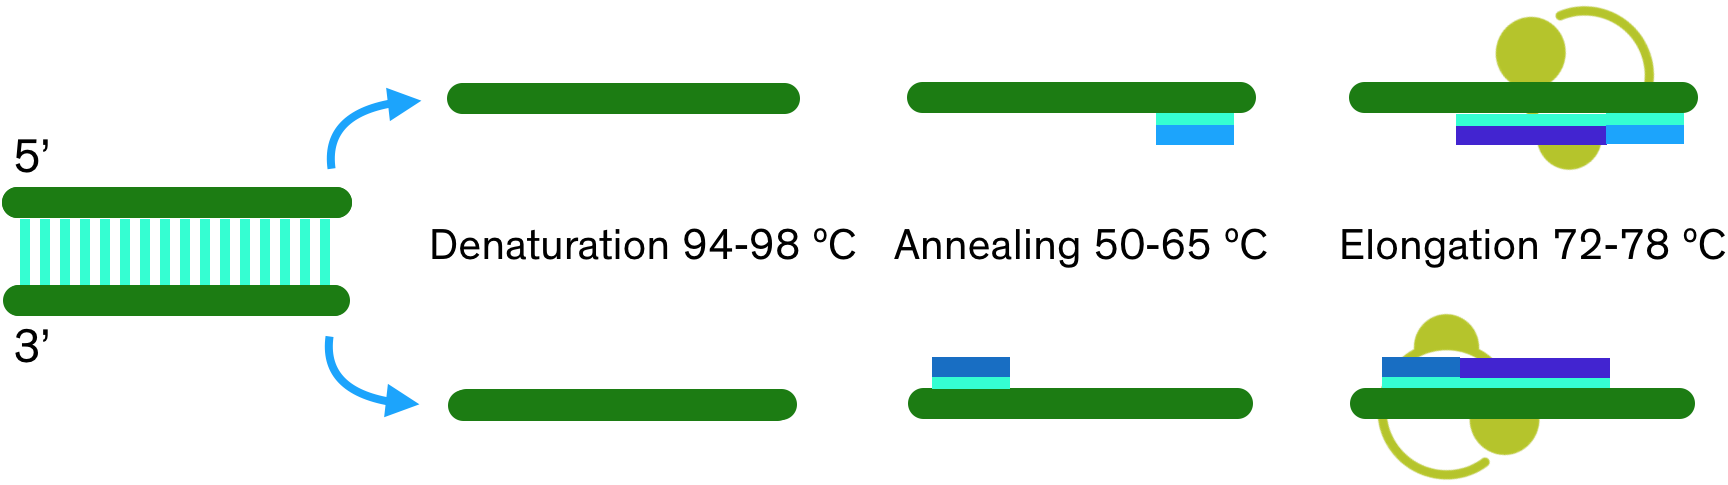
\includegraphics[scale=.4]{picto_PCR2}}
%     \end{center}
    
% \end{frame}

\begin{frame}
	\frametitle{Polymerase Chain Reaction (PCR)}
	\begin{figure}
	    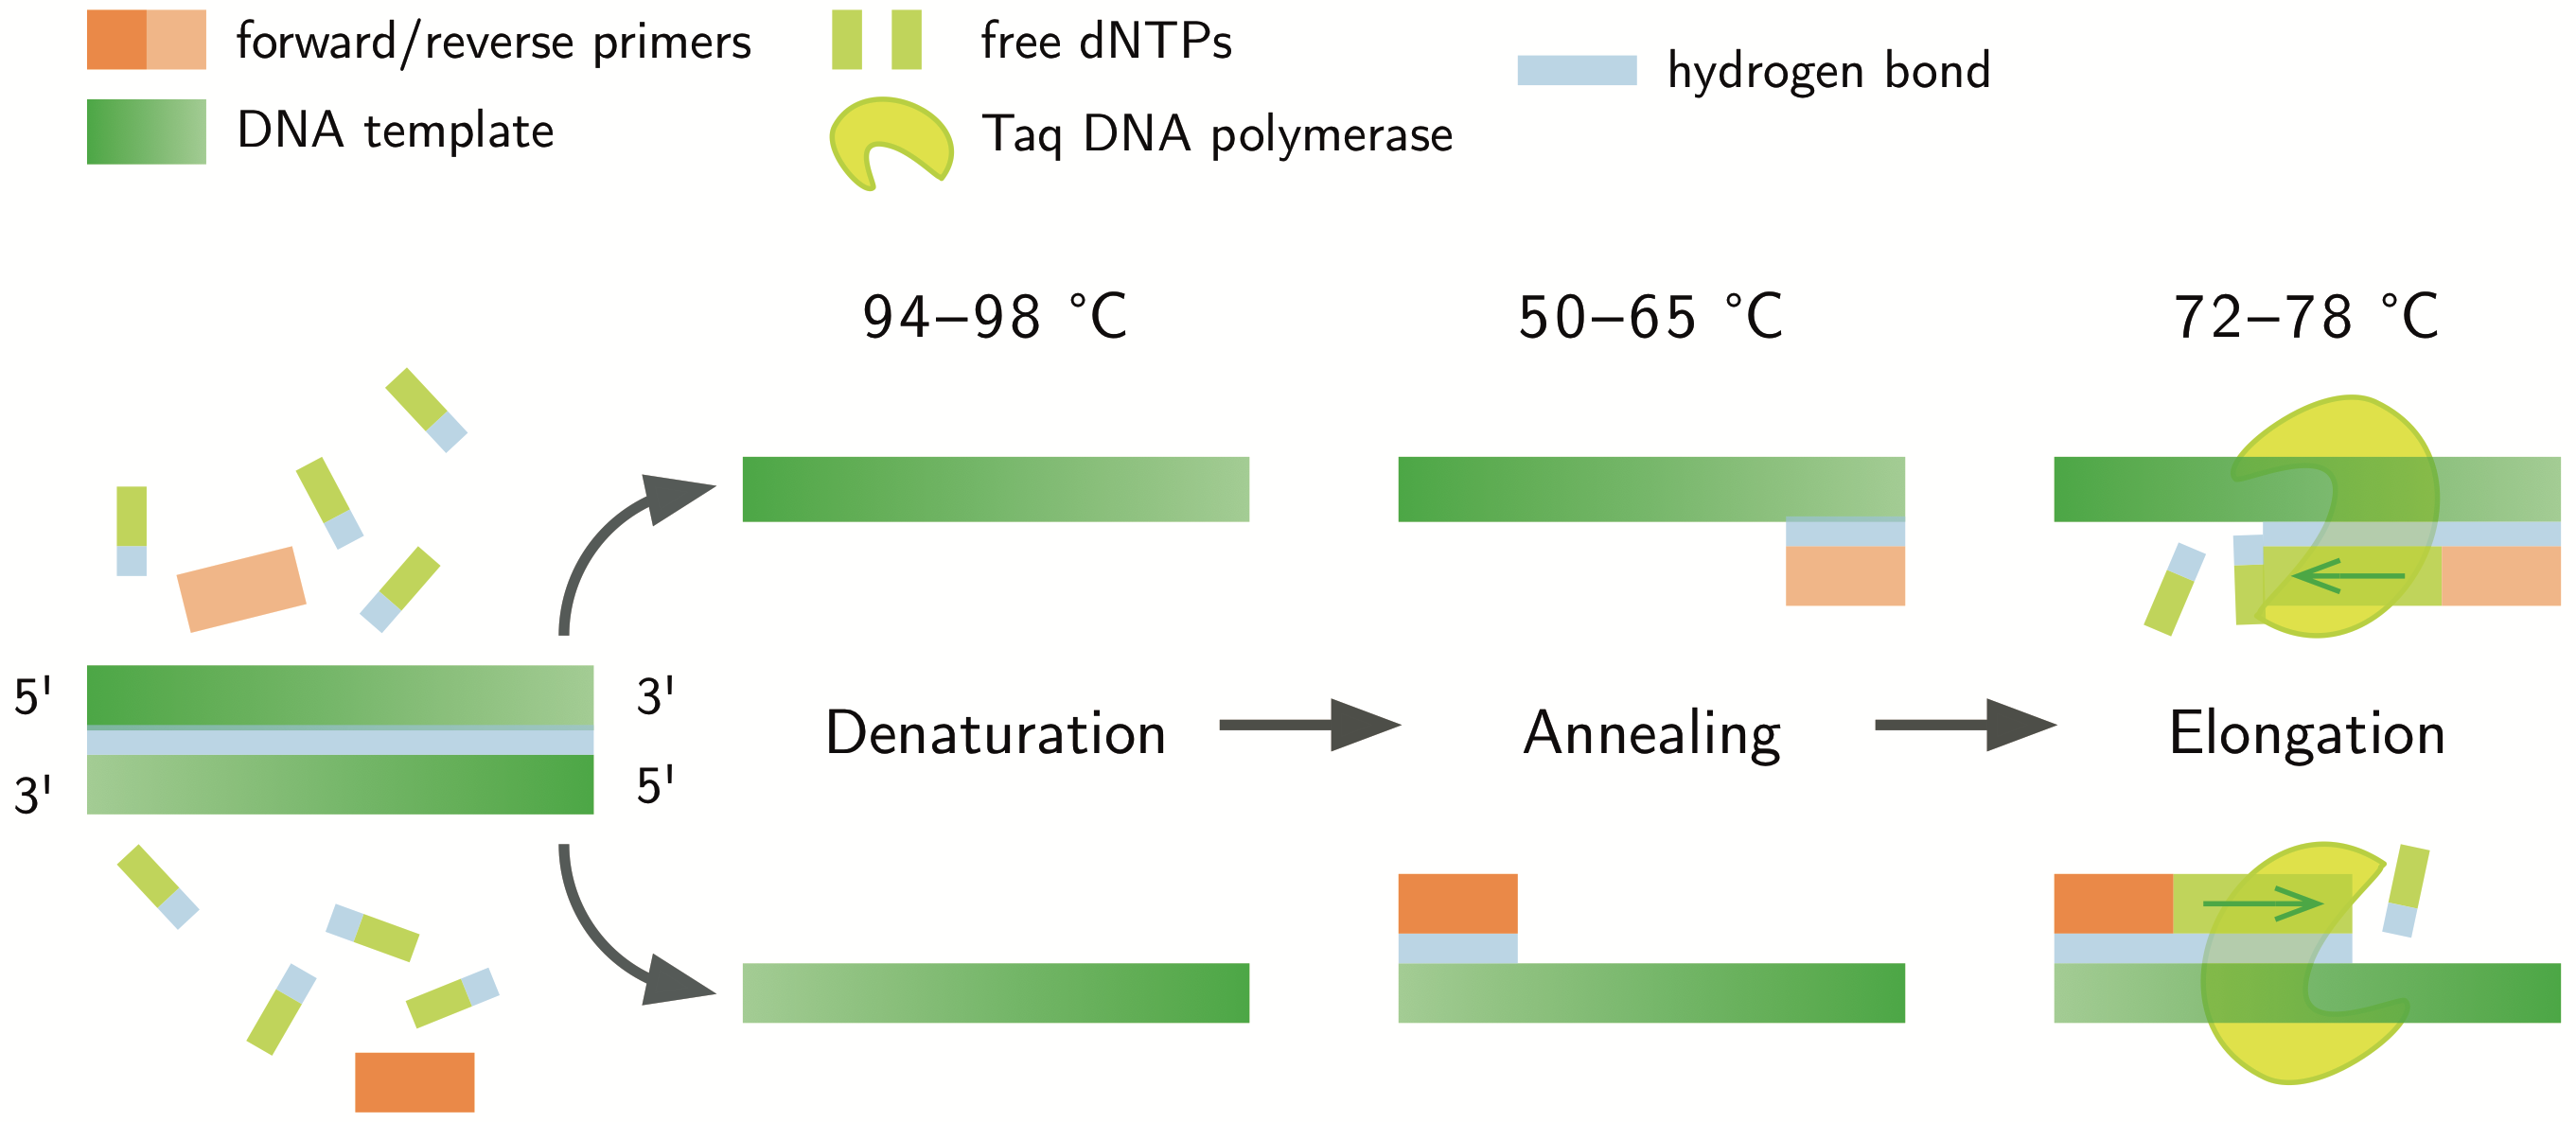
\includegraphics[scale=.7]{PCR}
	\end{figure}
\end{frame}


% A PCR has 3 phases which are executed repeatedly in a programmable thermal cycler.
% A phase is defined by keeping the temperature at a certain level to facilitate certain molecular reactions.
% [1] If we imagine the double-stranded DNA unwound, we can see the hydrogen bonds, which must be dissolved to allow polymerase-binding and promote copying.
% By increasing the temperature of the mixture the double-stranded DNA dissociates into single-stranded DNA [2]. This is the denaturation phase [3].
% [4] By cooling down the mixture we achieve that fwd and rev primers anneal to complementary regions [5].
% Then the temperature is slightly increased [6] to promote DNA synthesis by the polymerase [7]
% [8] The polymerase builds in freely available dNTPs by extending the primer sequences and producing a template-complementary sequence.
% This process is stopped by increasing the temperature again for dissociation. For the next cycle we have duplicated the number of templates, that is, we have the original genomes and the first generation of barcode copies.
% And a new cycle can start.

\begin{frame}
	\frametitle{Multiplex PCR}
	Multiplexing: add multiple distinct primer pairs for simultaneous amplification of many regions\\
	Challenges
    \begin{multicols}{2}
	\begin{enumerate}
	    \item Dimerization between $P$ primer sequences $$O(P^2)$$ % in the number of sequences
	    \item Sequence selection - exponentially many choices for a pool of $N$ multiplex primers $$\binom{N}{P}$$
	    \item Non-convex fitness landscape % when altering pool composition -- serious interactions
	 \end{enumerate}
	 \columnbreak
	 \begin{figure}
     \begin{subfigure}
         \centering 
         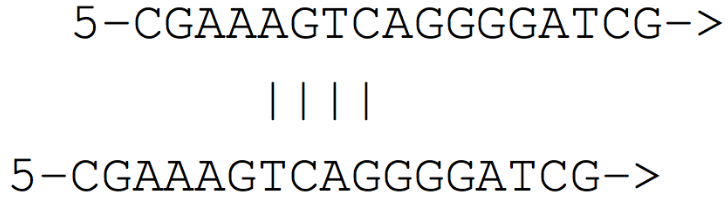
\includegraphics[width=.3\textwidth]{annealing_conn_fwd}
        %  \caption{Continuous annealing pattern.}
     \end{subfigure}
     \hfill
     \begin{subfigure} %[b]{0.5\textwidth}
         \centering
         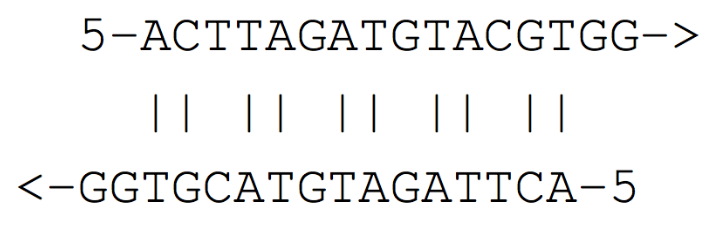
\includegraphics[width=0.3\textwidth]{annealing_disconn_rev}
    % \caption{Annealing patterns.}
     \end{subfigure}
    %  \caption{Examples of a connected and disconnected annealing pattern.}
     \begin{subfigure} %[b]{0.5\textwidth}
         \centering
         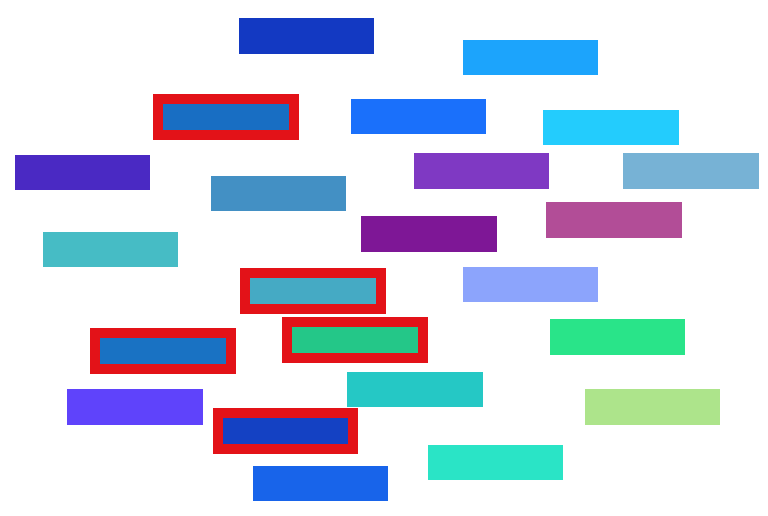
\includegraphics[width=0.25\textwidth]{picto_primerpool}
        %  \caption{.}
     \end{subfigure}
     \end{figure}
\end{multicols}
\end{frame}

% \begin{frame}\frametitle{Optimization a Loss Function}
% Goal: Minimize a loss function $L$ w.r.t. to a configuration $\theta$
% $$ 
% \widehat{\theta} = \arg\min_{\theta} L(\theta)
% $$
% \begin{multicols}{3}

% TODO: pic convex
% \columnbreak non-convex,
% \columnbreak
% discrete and non convex
% \begin{itemize}
%     \item Simulated Annealing 
% \end{itemize}
% \end{multicols}
% \end{frame}

% it is computationally intractable to optimize for larger values of n and p, e.g., authors use for p = 192 and more than 700 
\begin{frame}[fragile]\frametitle{Optimization Method: Simulated Annealing}\framesubtitle{via Stochastic Sampling}
Goal: Minimize a energy $E$ (or loss $L$) w.r.t. to a configuration $\theta$
$$ 
\widehat{\theta} = \arg\min_{\theta} E(\theta)
$$
% \begin{multicols}{2}
% Method of choice when optimization problem is
% 		\begin{itemize}
% 		    \item Computationally intractable % problem in which the only exact solution is one that takes too many resources (time, memory, etc.).
% 		    \item Non-convex target function
% 		\end{itemize}

% \columnbreak
\begin{algorithm}[H]
% \caption{Pseudocode Simulated Annealing}
\begin{algorithmic}[1]
\STATE $S = S_0$
\FOR{$g=1$ to $g_t$}
\STATE $T = \text{temperature}(1 - (g+1) / g_t)$ 
\STATE $S_{\text{new}} = \text{neighbor}(S)$
\IF{$P(E(S), E(S_{new}), T) \geq \text{random}(0, 1)$}
    \STATE $S = S_{\text{new}}$
\ENDIF
\ENDFOR
\RETURN $S$
\end{algorithmic}
% label{alg:seq}
\end{algorithm}

    % Let s = s0
    % For k = 0 through kmax (exclusive):
    %     T ← temperature( 1 - (k+1)/kmax )
    %     Pick a random neighbour, snew ← neighbour(s)
    %     If P(E(s), E(snew), T) ≥ random(0, 1):
    %         s ← snew
    % Output: the final state s
% \end{multicols}

\end{frame}


\section{Algorithm}
\begin{frame}\frametitle{SADDLE: Loss Function and Initialization}
% TODO: as pictogram
% Given: pool of candidates of forward (\pfwd) and reverse primers (\prev) for each gene target
\begin{enumerate}
    \item Selection of an initial primer set $S_0$ from candidate pool
    \item Evaluation of the Loss function $L(S_0)$
\end{enumerate}
\begin{eqnarray}
    L(S) &=& \sum_{b\geq a} Badness(p_a, p_b)\\
    Badness(p_a, p_b) &=& \sum_{q\in Q_a \cap Q_b} \frac{2^{|q|} 2^{\text{GC}}}{(d_a + 1)(d_b + 1)}\\
    Q&=&\{ q\in p: | q| \in [4;8]\}
\end{eqnarray}
Note: hashing of patterns reduces runtime to $\mathcal{O}(PN)$ per time step
\end{frame}

\begin{frame}\frametitle{SADDLE: Repeat Steps 3 and 4} % until acceptable primer set $S_{\text{final}}$ is constructed
\begin{enumerate}
    \setcounter{enumi}{2}
    \item Generate temporary primer set $T$ based on set $S_g$ (primer set from generation $g$) by randomly changing 1 or more primers
    \item Evaluate $L(T)$, and set $S_{g+1}$ to either $S_g$ (no change) or $T$:
    \begin{description}
        \item[case $L(T) < L(S_g)$] then $S_{g+1} = T$
        \item[case $L(T) \geq L(S_g)$\footnote{and $g \leq g_T$}] then $S_{g+1} = T$ with $P = exp\{\sfrac{L(S_g) - L(T)}{C(g)}\}$
        \item[otherwise] stochastic gradient descent (SGD), i.e., $S_{g+1} = S_g$
    \end{description}
    
\end{enumerate}
Notes: Probability $P(\cdot)$ depends on
\begin{itemize}
    \item $p$ depends on magnitude $L(S_g) - L(T)$ % of detriment
    \item generation-dependent and decreasing function $C(g)$
\end{itemize}
\end{frame}

%----------- MAIN RESULTS ------------------------------
\section{Evaluation}
\begin{frame}{Evaluation I -- Paper}\framesubtitle{96-plex primer set selected from cancer-related genes}
% Design and experimental evaluation of a 96-plex primer set zarbitrarily selected exon of a different cancer-related gene
\begin{figure}
    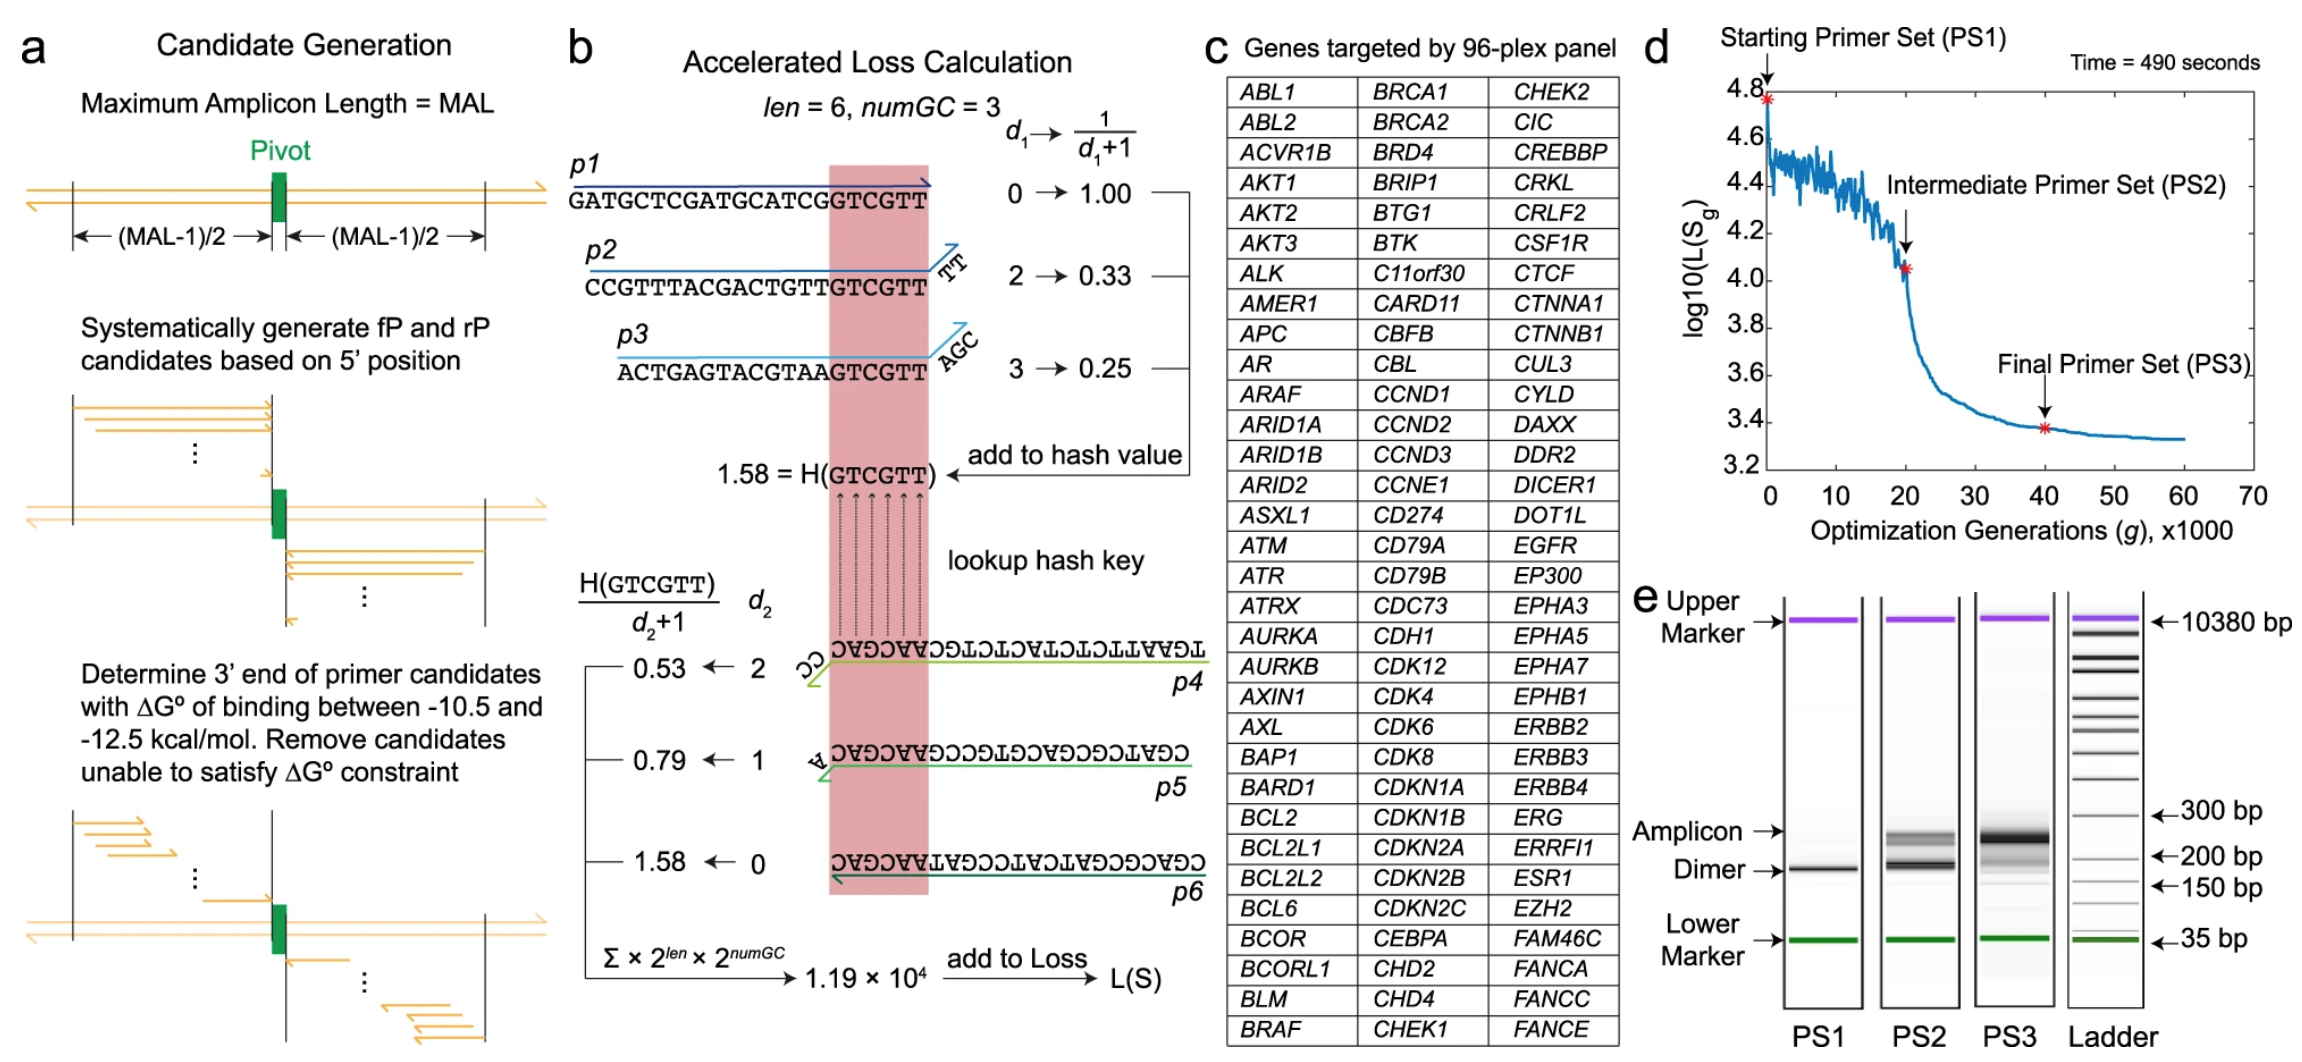
\includegraphics[width=\textwidth]{fig2_paper}
    \caption{Evaluated on 10 ng of NA18562 human genomic DNA.}
\end{figure}

\end{frame}

\begin{frame}{Results I -- Paper}\framesubtitle{Paper}\framesubtitle{96-plex primer set selected from cancer-related genes}
\begin{figure}
    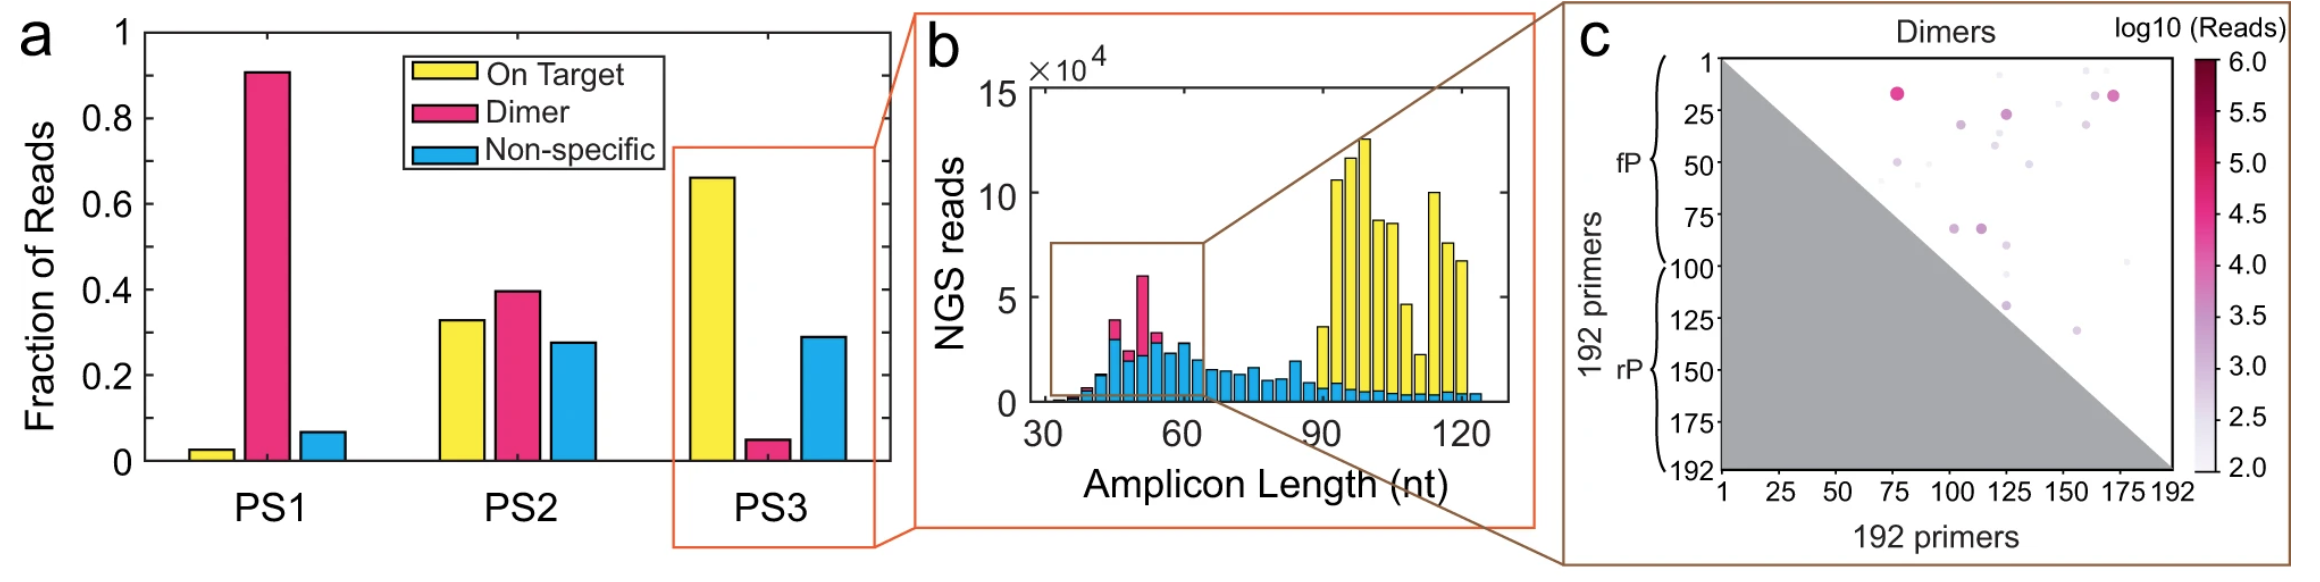
\includegraphics[width=\textwidth]{fig3_top_paper}
    \caption{Read analysis. {\bf On Target} -- aligned to intended amplicon, {\bf Dimer} -- primer dimers, {\bf Non-specific} -- other}
\end{figure}

\hrulefill\\
{\it in silico} upscale demo with 384 amplicon panel (768 primers) on 40 ng NA18562 genomic DNA:
\begin{itemize}
    \item On-Target 43 \%,  Non-specific 56 \%, and 1 \% dimer amplicons
\end{itemize}
\end{frame}

\begin{frame}
	\frametitle{Evaluation II}\framesubtitle{Prediction Accuracy of the Badness function}
	\begin{figure}
    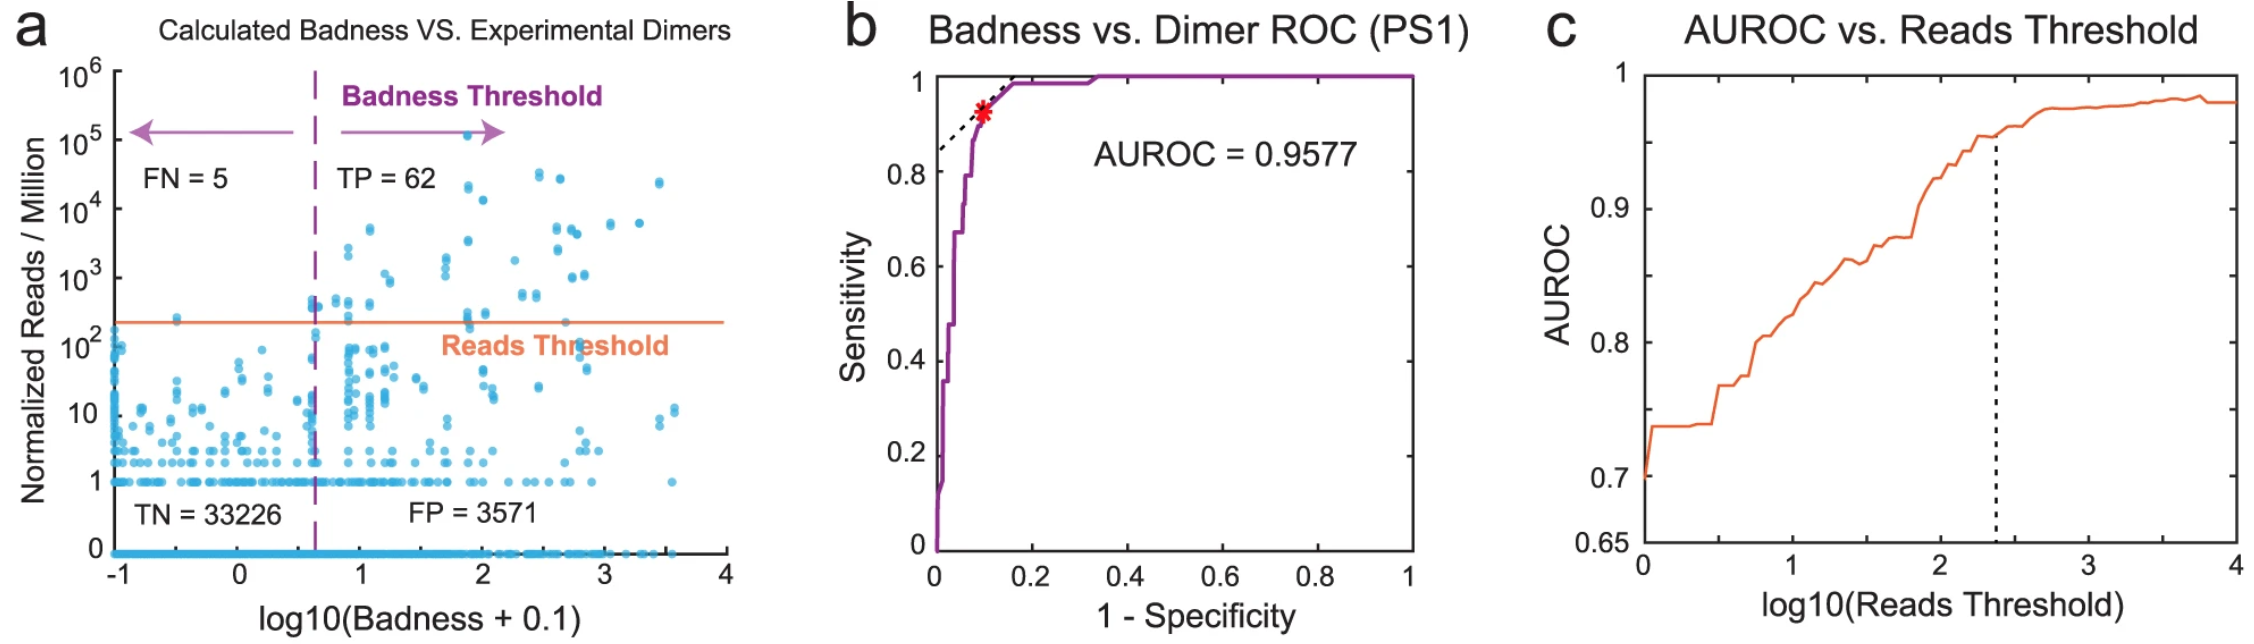
\includegraphics[width=\textwidth]{fig4_top_paper}
    \caption{{\bf a} Observed vs. predicted primer dimers. Reads threshold here: mean on-target read depth. {\bf b} ROC Sensitivity vs. 1 - Specificity by shifting Badness threshold. \textbf{c} AUROC dependency of reads threshold.}
\end{figure}
Current setting: 92.5 \% sensitivity and 90.3 \% specificity
\end{frame}

\begin{frame}
	\frametitle{Evaluation II}\framesubtitle{Metabarcoding of Plankton}
	%\justifying
% 	Goal: trade-off coverage and resolution
    \begin{enumerate}
        \item Compute primer sequences on 19 plankton clades \cite{PriSeT2021}
        \item Select proto-primers for head of Gibb's: $\Delta G \in [x_{\alpha_{5\%}}:x_{\alpha_{95\%}}]$ \footnote{$x_{\alpha_c}: cdf(x_{\alpha_c}) = c$} %.95-quantile  and drop .5-quantile for Free Gibbs energy (show density plot)
        \item Use SADDLE to propose multiplex primers (iteration vs. loss plot)
        
        \item Result: [Live Session or recorded animation (see attachment)]
    \end{enumerate}
	
\vspace*{\fill}
Code: \url{https://github.com/mariehoffmann/PriSeT_X_SADDLE}
\end{frame}

\begin{frame}
	\frametitle{Evaluation II -- Metabarcoding of Plankton}\framesubtitle{Tuning Acceptance Probability -- Standard Error}
\begin{eqnarray}
P(S_g = T | L(T) > L(S_g)) &=& \exp{(L(S_g) - L(T)) \cdot \text{stderr}^{-1}} \\
\text{stderr}&=&\frac{\sigma}{\sqrt{p}}
\end{eqnarray}	
\begin{figure}
    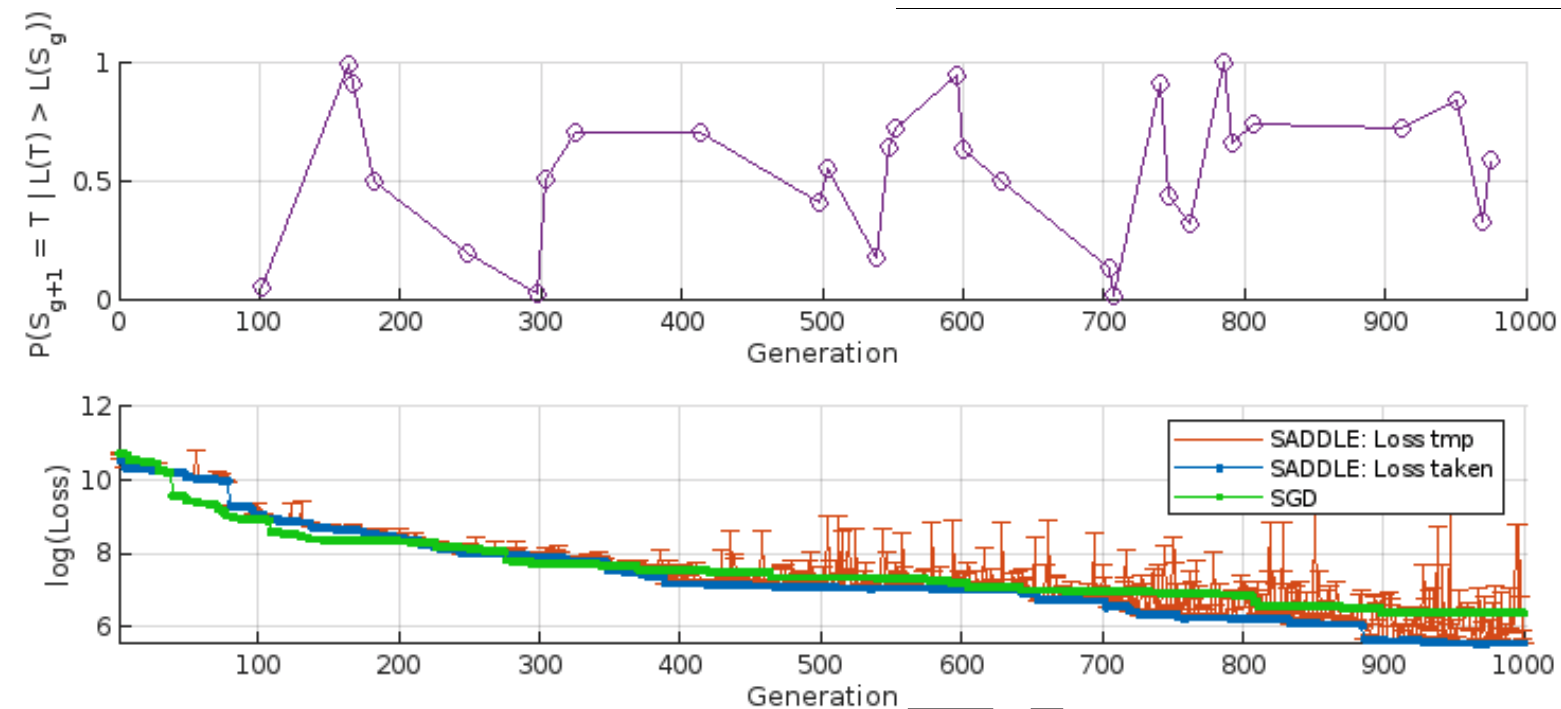
\includegraphics[width=.7\textwidth]{plankton_p64_gt100_gT150_eps001_Pc}
    \caption{$N = 436$, $P = 64$, detriment normalized via stderr}
\end{figure}
\end{frame}

% \begin{frame}
% 	\frametitle{Evaluation II -- Metabarcoding of Plankton}\framesubtitle{Tuning Acceptance Probability -- Standard Error}
% \begin{eqnarray}
% P(S_g = T | L(T) > L(S_g)) &=& \exp{(L(S_g) - L(T)) \cdot \text{stderr}^{-1}} \\
% \text{stderr}&=&\frac{\sigma}{\sqrt{p}}
% \end{eqnarray}	
% \begin{figure}
%     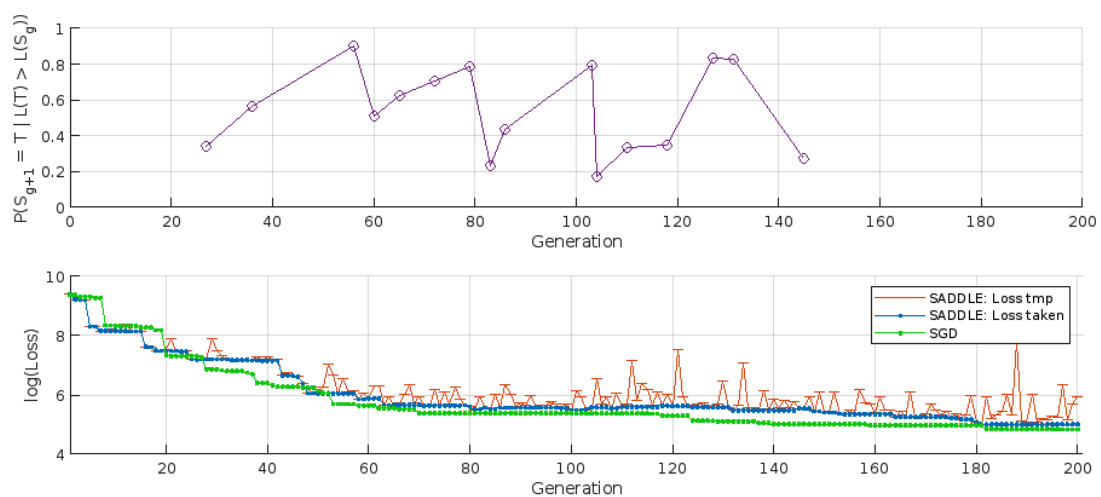
\includegraphics[width=.7\textwidth]{plankton_p24_gt100_gT150_eps001_Pc}
%     \caption{$N = 436$, $P = 24$, detriment normalized via stderr}
% \end{figure}
% \end{frame}

\section{Discussion}
\begin{frame}\frametitle{Discussion}
\begin{enumerate}
    \item Baseline SGD can be better
    \begin{itemize}
        \item Run with $P(\cdot)$, and SGD for comparison
        \item Repeat with different seeds of RNG
        \item Run sufficiently many iterations
    \end{itemize}
    \item Plenty of constraints unchecked
    \begin{itemize}
    \item forward complementary, disconnected annealing patterns, $(A|T)$-tails, hairpins, etc.
    \item Need better understanding of primer dimerization: high-ranked dimers from experiment had low badness score and vice versa % some long patterns with high pred. badness did not occur in high ranks of practical experiment
    \end{itemize}
    \item Parameter tuning $C_g$ for acceptance probability difficult
    \begin{itemize}
        \item Needs robustness based on Loss statistics
    \end{itemize}
    \item Control for proportion of fwd/rev primers
\end{enumerate}
\end{frame}


\begin{frame}\frametitle{Conclusion}
\begin{enumerate}
    \item SADDLE reduces reagent costs while amplifying hundreds of target templates simultaneously
    \item Broad Applicability of Framework
    \begin{itemize}
       \item Different types of PCR
        \item Amplification of multiple regions of same genome
        \item Gene fusion detection
        \item Amplification of similar regions in different genomes
    \end{itemize}
    \item Framework adjustable, e.g., Metabarcoding -- identification of many phylogenetically diverse species % enforce high resolution by
        \begin{enumerate}
            \item Sample Clade index $j$
            \item Sample primer pair from Clade$_j$ for probabilistic exchange
        \end{enumerate} 
    \item More sequence checks can be easily added with low computational overhead (C++)
\end{enumerate}
\nocite{Xie2022, PriSeT2021}
\end{frame}

%----------- REFERENCES  -------------
%----------- No editing in references section ----------
%----------- edit only in References.bib ----------
	\begin{frame}[allowframebreaks]
		\justifying
		\frametitle{List of References}
		\printbibliography
	\end{frame}


\begin{frame}\frametitle{Appendix: Evaluation I}
\begin{figure}
    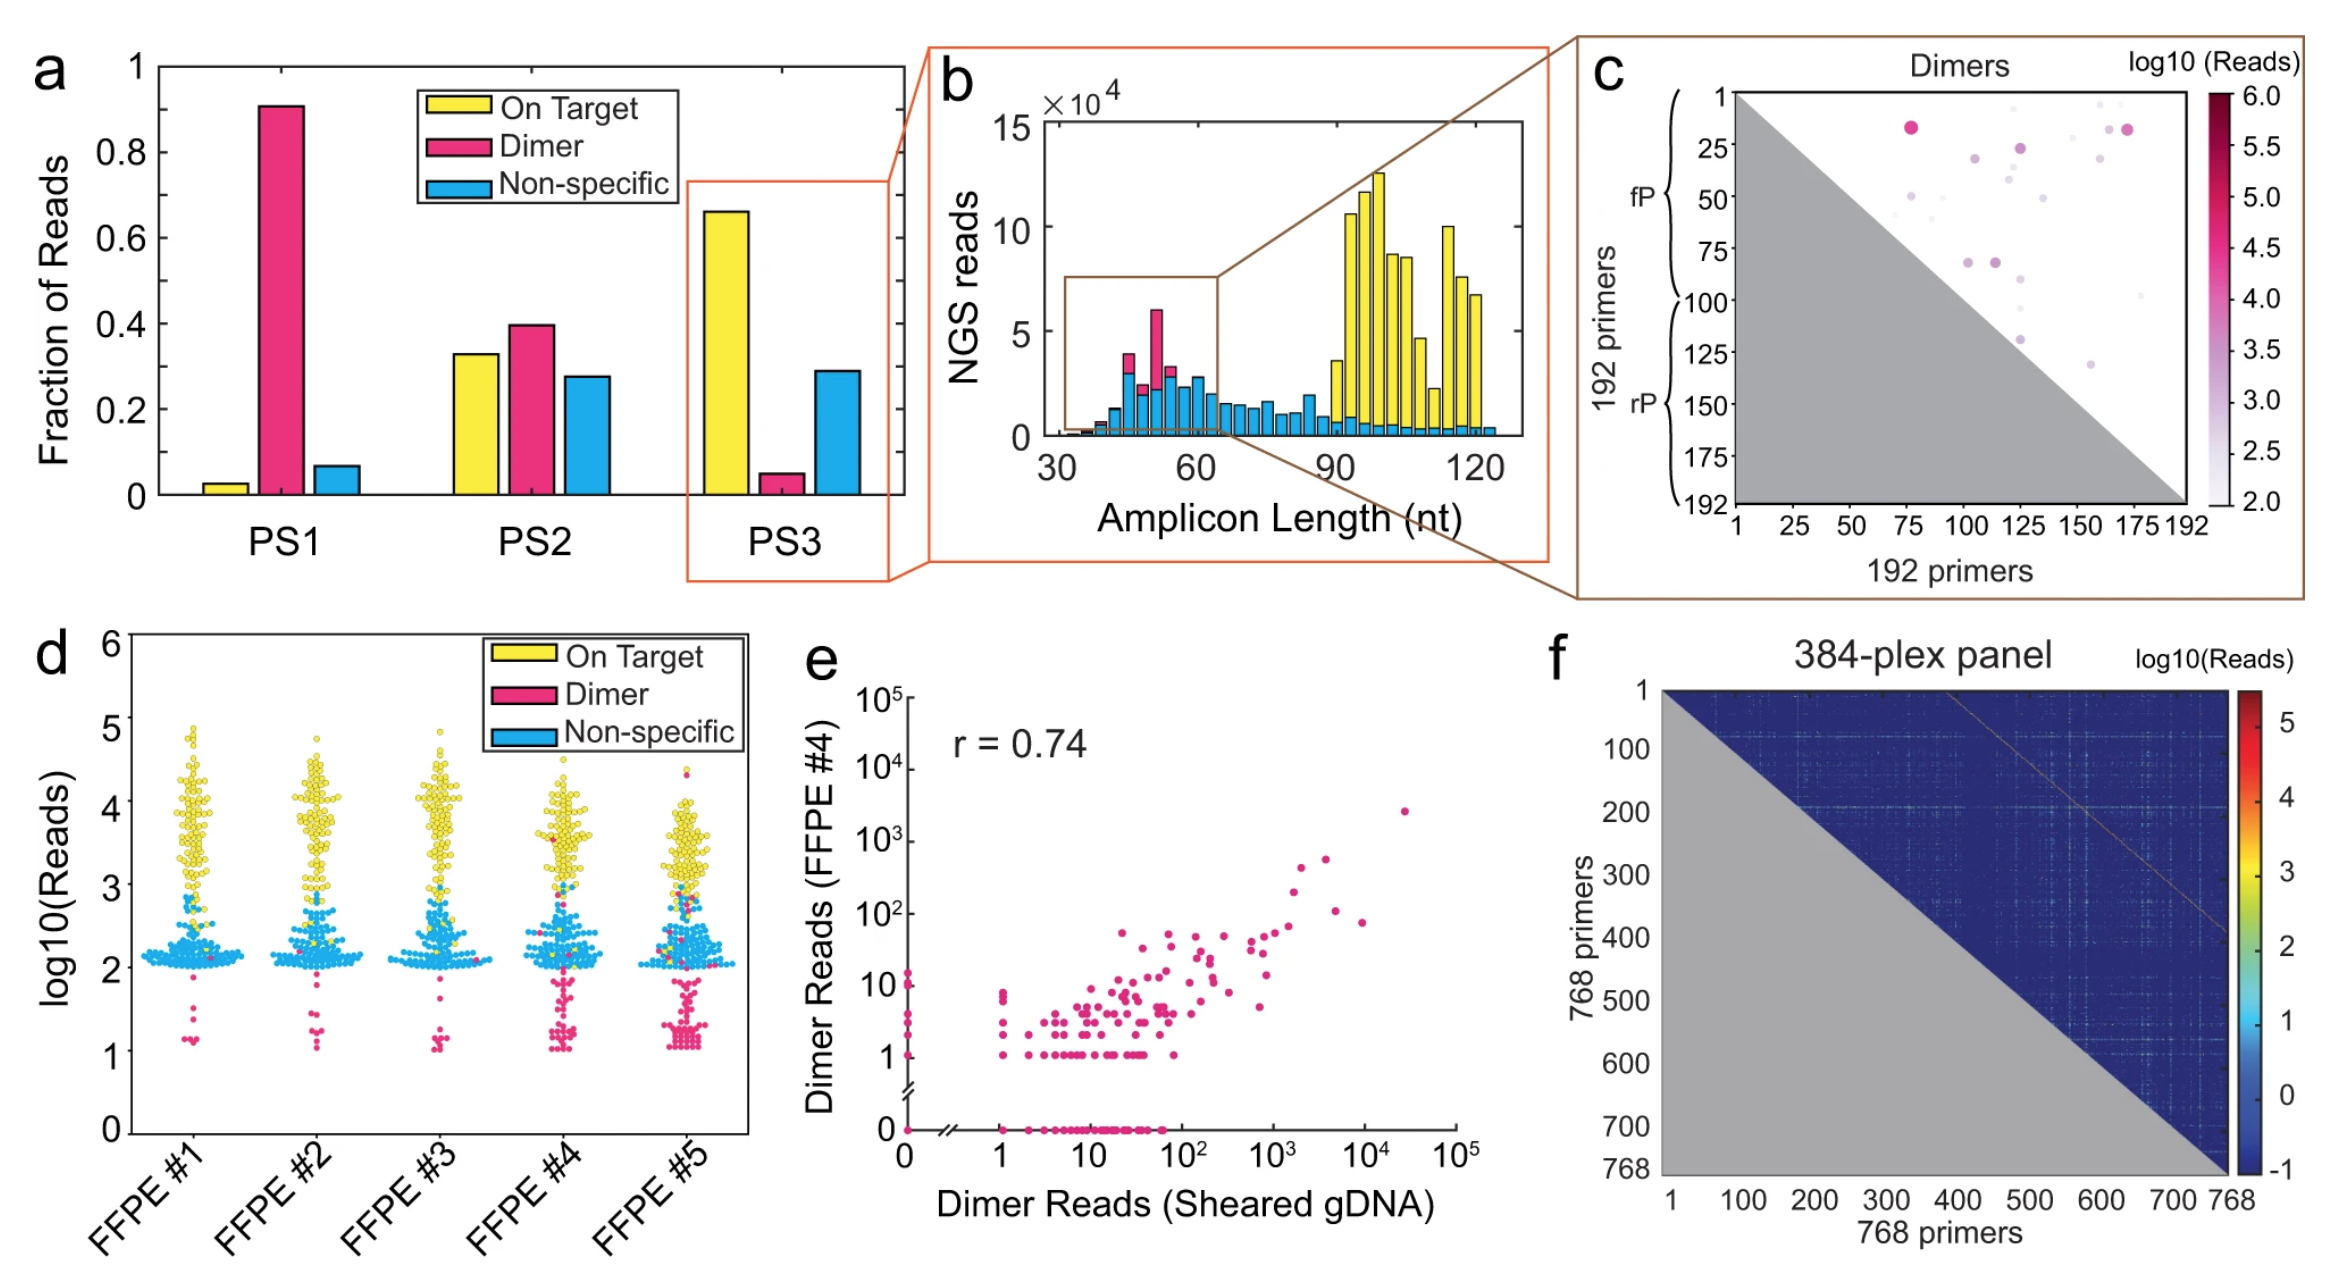
\includegraphics[width=\textwidth]{fig3_paper}
    % \caption{}
\end{figure}
\end{frame}

\begin{frame}\frametitle{Appendix: Evaluation II}
\begin{eqnarray}
P(S_g = T | L(T) > L(S_g)) &=& \exp{(L(S_g) - L(T)) \cdot \text{stderr}^{-1}} \\
\text{stderr}&=&\frac{\sigma}{\sqrt{p}}
\end{eqnarray}	
\begin{figure}
    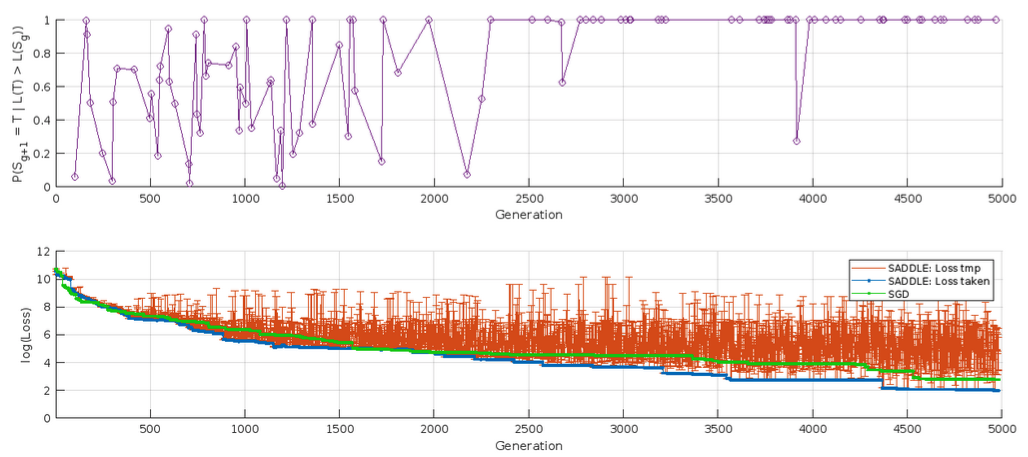
\includegraphics[width=.7\textwidth]{plankton_p64_gt5k_gT5k_eps001_Pc}
    \caption{$N = 436$, $P = 64$, detriment normalized via stderr, $g_t = 5000$, $g_T = 5000$, $log(L^{\text{SADDLE}}_{g_T}) = 7.3$, $log(L^{\text{SADDLE}}_{g_T}) = 16.1$}
\end{figure}

\end{frame}

%----------------------------------------------------
\end{document}
